\documentclass[a4paper,11pt,headinclude=true,headsepline,parskip=half,DIV=13]{scrartcl}

% font, style, etc.
\usepackage[utf8]{inputenc} % defines
\usepackage[automark]{scrlayer-scrpage}
\usepackage{csquotes}
\usepackage{xspace} % proper space after macros with 0 args

% mathematics
\usepackage{amsmath}
\usepackage{amssymb}

% figures, tables, etc.
\usepackage{hyperref} %
\usepackage{graphicx}
\usepackage{tikz}
\usepackage{pgf}
\usepackage{xcolor}
\usepackage{placeins} % -> floatbarrier
\usepackage{siunitx}  % -> handling of units
%\usepackage[printwatermark]{xwatermark}
%\newwatermark[allpages,color=red!50,angle=45,scale=1.8,xpos=0,ypos=0]{\textsf{DRAFT ONLY,NOT APPROVED}}

% code
\usepackage{listings}
\lstset{
language=Python, 
backgroundcolor = \color{light-gray},
basicstyle=\scriptsize\sffamily,
stringstyle=\color{orange},
breaklines=true,
numberstyle=\tiny\color{gray},
keywordstyle=\bfseries\color{dark-blue}\textit, % print keywords dark-blue
commentstyle=\color{dark-green}, % print comments dark-green
showstringspaces=false} % spacing between strings not showed

\newcommand{\listcode}[3]{\lstinputlisting[numbers=left,firstnumber=#1,firstline=#1,lastline=#2]{#3}}
\newcommand{\listcodeplot}[2]{\listcode{#1}{#2}{../sim/01_car_example_plotting.py}}
\newcommand{\listcodeanim}[2]{\listcode{#1}{#2}{../sim/02_car_example_animation.py}}

% others
\usepackage{acronym}
\usepackage{luacode}
\usepackage{soul}

% bibliography
\usepackage[style=verbose-ibid,backend=bibtex]{biblatex}
\bibliography{literature}

% theorems
\newtheorem{defi}{Definition}[section]

% setup the appearance of links
\hypersetup{
    colorlinks = true, % false -> red box arround links (not very nice)
    linkcolor={blue!100!black},
    citecolor={blue!100!black},
    urlcolor={blue!100!black},
}

% manage glossaries
% Call makeglossaries on a command prompt after LaTeX compiling,
% the re-run LaTeX
\usepackage{glossaries}
\setacronymstyle{long-short}
\makeglossaries
\newacronym{ivp}{IVP}{initial value problem}
\newacronym{ode}{ODE}{ordinary differential equation}

% define shortcuts
\newcommand{\ad}{\mathrm{ad}}
\renewcommand{\d}{\mathrm{d}} % d vor differential forms
\newcommand{\NV}{{\cal N}\,}
\newcommand{\rang}{\mathrm{rang}}
\newcommand{\im}{\mathrm{im}}
\newcommand{\spann}{\mathrm{span}}
\newcommand{\R}{\mathbb{R}} %  set of real numbers
\newcommand{\py}{\emph{Python}\xspace}
\newcommand{\scipy}{\emph{SciPy}\xspace}
\newcommand{\numpy}{\emph{NumPy}\xspace}
\newcommand{\mpl}{\emph{Matplotlib}\xspace}
\newcommand{\uu}{\mathbf{u}}
\newcommand{\f}{\mathbf{f}}
\newcommand{\x}{\mathbf{x}}
\newcommand{\y}{\mathbf{y}}
\newcommand{\z}{\mathbf{z}}
\newcommand{\xZero}{\mathbf{x}_0}

% color definitions
\definecolor{light-gray}{gray}{0.95}
\definecolor{dark-blue}{rgb}{0, 0, 0.5}
\definecolor{dark-red}{rgb}{0.5, 0, 0}
\definecolor{dark-green}{rgb}{0, 0.5, 0}
\definecolor{gray}{rgb}{0.5, 0.5, 0.5}

% Avoid ugly indentations in footnotes.
\deffootnote[1em]{1em}{0em}{%
\textsuperscript{\thefootnotemark}%
}

\luadirect{dofile("luainputlisting.lua")}
\newcommand*\luainputlisting[2]{
    \luadirect{print_listing(\luastring{#1}, \luastring{#2})}
}

% ----------------------------------------------------------------------------
\subject{\py for simulation, animation and control}
\title{Design and Simulation of LQR Control}
\subtitle{An introductory tutorial for the design and implementation of LQR controllers for time-invariant and time-variant linear systems}
\author{Robert Heedt\thanks{Institute for Control Theory, Faculty of Electrical and Computer Engineering, Technische Universität Dresden, Germany} \and Jan Winkler\footnotemark[1]}
\publishers{}
\date{\today}
% ----------------------------------------------------------------------------

% Headings
\pagestyle{scrheadings}
\ihead{\leftmark}
\chead{}
\ohead{Page \pagemark}
\ifoot{}
\cfoot{Python Control Tutorial 4}
\ofoot{}

\begin{document}

\maketitle




\tableofcontents

\newpage

\section{Introduction}
The goal of this tutorial is to teach the usage of the programming language \py as a tool for developing and simulating control systems.
The following topics are covered:
\begin{itemize}
    \item Flatness based feedforward control using existing trajectory generators
    \item Feedback control using LQR for linear time-invariant (LTI) system
    \item Demonstration of problematic situations
    \item Feedback control using LQR linear time-variant (LTV) system
\end{itemize}
Later in this tutorial this process is applied to design control strategies for the swingup of a cart-pole system.

\section{Implementing the System}
In order to demonstrate the design methods discussed in the following, a simple academic example\autocite{ludyk} will be used.
The system state~$x=(x_1, x_2)$ has two components and the scalar input is called~$u$.
Written in state-space-form, the system equation then is:
\begin{equation}
\dot x = F(x, u) = 
\begin{pmatrix}
a \sin(x_2)\\
-x_1^2+u\\
\end{pmatrix}\,.
\label{eq:academic_example_ss}
\end{equation}
Later, the jacobians
\begin{equation}
A^*(x^*, u^*) := \left.\frac{\partial F}{\partial x}\right\vert_{(x^*, u^*)}= \begin{pmatrix}0 & a \cos(x^*_2)\\-2 x^*_1 & 0\end{pmatrix}
\label{eq:jac_A}
\end{equation}
and
\begin{equation}
B^*(x^*, u^*) := \left.\frac{\partial F}{\partial u}\right\vert_{(x^*, u^*)}= \begin{pmatrix}0 \\ 1\end{pmatrix}
\label{eq:jac_B}
\end{equation}
will also be needed.

Implementing this system in Python then simply means expressing these terms as functions containing these computations. 
\luainputlisting{../sim/01_lqr.py}{defsystem}
Notable are mainly the usage of NumPy arrays for all vectors and the \lstinline{Parameters} class, please refer to a previous tutorial if unsure about these aspects.

\section{Trajectory Planning and Feedforward}

Similar to previous tutorials, feedforward control design can be simplified significantly by exploiting the flatness property of this system.
Specifically, the flat output is~$y=x_1$.
Recall, this means a desired trajectory $t \mapsto x_1^*(t)$ can be freely chosen (as long as it is sufficiently often differentiable).
Then, the trajectories for all other system variables (states and inputs) is calculated analytically without integration.

To this effect, the first system equation in~\eqref{eq:academic_example_ss} is solved for~$x_2$, yielding
\begin{equation}
x_2 = \arcsin\left(\frac{\dot x_1}{a}\right)
\label{eq:flatness_x2}
\end{equation}
which also introduces the constraint~$\forall t: |\dot x_1(t)| \leq |a|$ to trajectory planning.

After differentiating~\eqref{eq:flatness_x2} w.\,r.\,t.\ time, resulting in
$$
\dot x_2 = \frac{\ddot x_1}{\sqrt{a^2-\dot x_1^2}}\,,
$$
a term for $u$ is obtained by solving the second component of~\eqref{eq:academic_example_ss}:
$$
u = \dot x_2 + x_1^2 =  \frac{\ddot x_1}{\sqrt{a^2-\dot x_1^2}} + x_1^2\, .
$$
For the \py implementation, the trajectory planner from a previous tutorial is reused to obtain a polynomial that transitions from~$y(t_0) = y_0$ to~$y(t_f) = y_f$.
This function is then evaluated at the time values stored in vector \lstinline{t_traj}.
\luainputlisting{../sim/01_lqr.py}{plantraj}
The previously derived formulas are then translated into NumPy operations to obtain the values for~$x_2$ and~$u$ at every time step.
\luainputlisting{../sim/01_lqr.py}{flatness}

\section{Linear Time Invariant Systems}
Before an LQR controller can be designed, the system in question must be linear.
As a rough approximation, Taylor linearization is used to obtain a linear time-invariant (LTI) system which is valid in the proximity to the operating point $(x^*, u^*)$.
In new coordinates $\tilde x=x - x^*$ and $\tilde u = u - u^*$ as well as by defining~$A:=A^*(x^*,u^*)$ and~$B:=B^*(x^*,u^*)$, the new state-space-form is then
$$
\dot{\tilde x}(t) = A \tilde x(t) + B \tilde u(t)\, .
$$
In \py, the operating point is defined by a time $t^*$ along the planned trajectory.
The corresponding array index is first determined and then used to get the values~$(x^*, u^*)$, with which the system matrices are computed.
\luainputlisting{../sim/01_lqr.py}{linsys}

Now an LQR controller will be designed by the book.
This means defining a cost-function
$$
J = \int_0^\infty \tilde x^T(t) Q x(t) + \tilde u^T(t) R u(t) \, \mathrm d t
$$
with the tuning matrices $Q$ and $R$ usually chosen as diagonal.
Minimizing this function leads to the algebraic Riccati equation
\begin{equation}
P A + A^T P - P B R^{-1} B^T P + Q = 0
\label{eq:riccati_are}
\end{equation}
having to be solved for $P$.
In \py the SciPy package fortunately contains the routine \lstinline{solve_continuous_are} which does exactly that.

The cost function then is minimal if a constant state feedback~$\tilde u = - K \tilde x$ is applied, with
$$
K = \begin{pmatrix} k_1 & k_2 \end{pmatrix} = R^{-1} B^T P\, .
$$
These computations -- save for the applying the actual control law, which happens in the main simulation loop -- can now be compactly written as
\luainputlisting{../sim/01_lqr.py}{solveare}

Now it is time to look at some simulation results.
Shown in Figure~\ref{fig:ludyk_lti} on the left side is the combination of feedforward control and feedback control, designed for a system linearized around the planned trajectory values at $t^*=0$.
The initial state~$x(0)$ is slightly offset from the planned initial position~$x^*(0)$, but the controller manages to track the trajectory anyway.

However, this choice of linearization point was arbitrary and lucky.
When e.\,g.\ $t^*=5$ is picked instead, the closed loop system immediately starts moving away from the reference value and tracking capability is lost.
This is demonstrated on the right side of Figure~\ref{fig:ludyk_lti}.

\begin{figure}[ht]
    \centering
    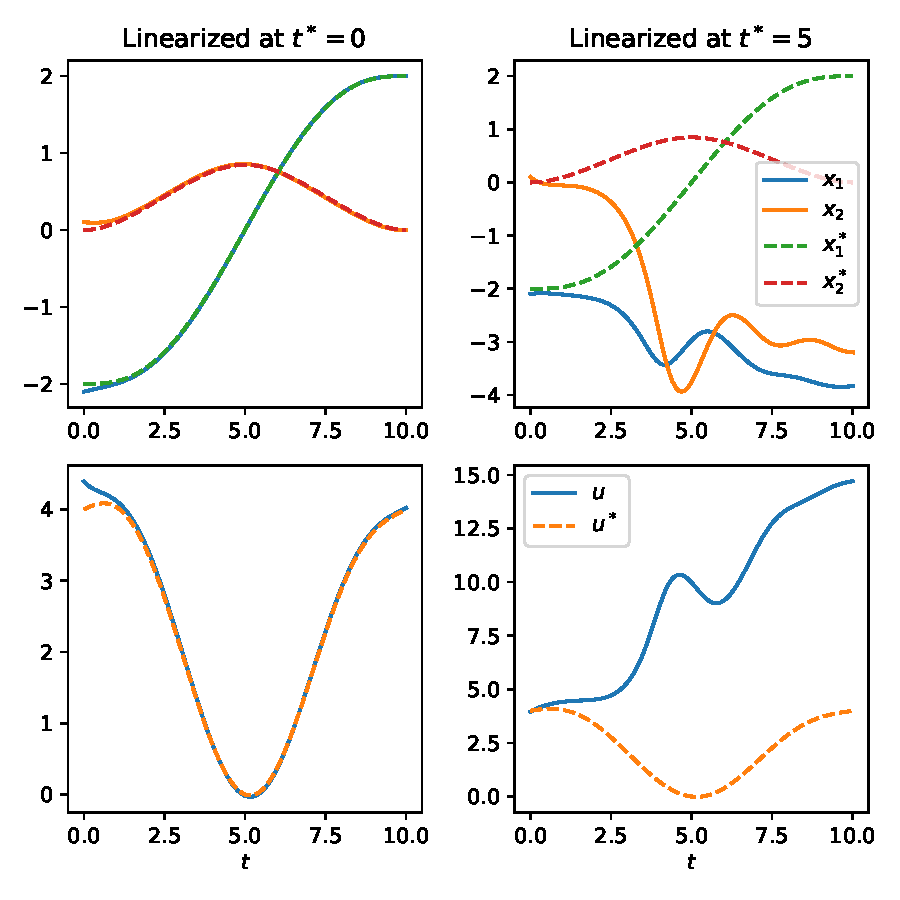
\includegraphics[scale=1]{img/ludyk_lti.pdf}
    \caption{Closed loop simulation of trajectory tracking, controller designed for different linearization points}
    \label{fig:ludyk_lti}
\end{figure}

In fact, simply sticking to $t^*=0$ also does not work.
For other reference trajectories, e.\,g.\ for~$y(0)=2$ and~$y(10)=-2$ (the reverse trajectory if you will), choosing the same linearization time fails.
In that case~$t^*=10$ must instead be used.

It appears that tracking arbitrary trajectories with this approach is not feasible, since the linearized system can never sufficiently represent the more involved non-linear dynamics and a "one size fits all" constant state feedback is therefore bound to fail.

One might be tempted to improve the controller by simply re-linearizing the system and re-computing the feedback matrix at every time step.
For this specific case this approach actually works and is very easy to implement when a normal LQR controller already exists.
Simulation results are shown in Figure~\ref{fig:ludyk_pseudoltv}, along with a plot of the changing feedback matrix entries over time.

\begin{figure}[ht]
    \centering
    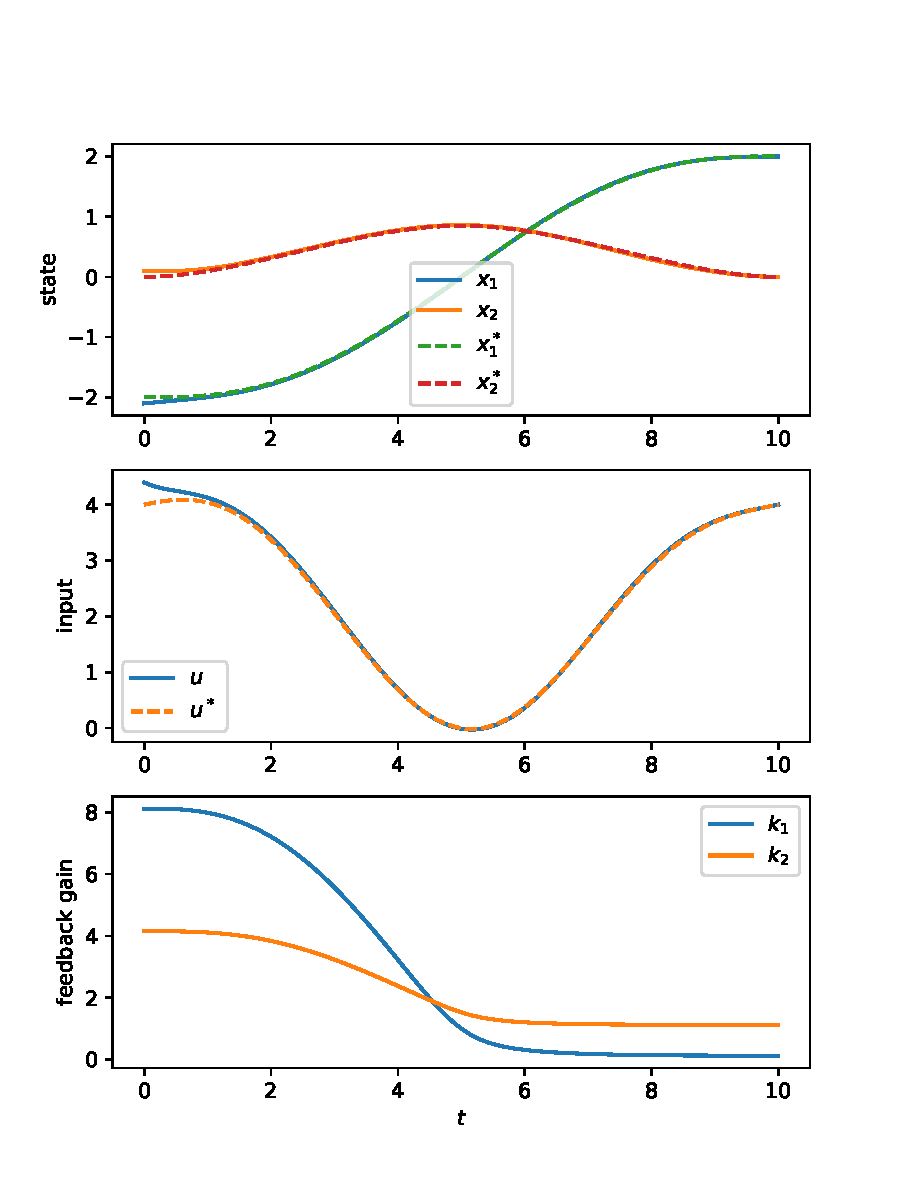
\includegraphics[scale=1]{img/ludyk_pseudoltv.pdf}
    \caption{Closed loop simulation of trajectory tracking, controller retuned for linearized system at every time step}
    \label{fig:ludyk_pseudoltv}
\end{figure}

Remember this is dangerous territory though.
No stability guarantees can be made here, because this ad-hoc solution corresponds to a linear system approximation with time-variant system matrices
$$
\dot{\tilde x}(t) = A(t)\tilde x(t) + B(t) u(t)\, .
$$
For a linear time-variant system, the closed loop system matrix $A(t) - B(t)K(t)$ must only contain eigenvalues $s$ with $\mathrm{Re}\,(s) < 0$, but also be \textbf{constant} in order for the closed loop to be stable!
This property is not ensured in this controller design, using it is therefore not recommended.

\FloatBarrier
\section{Linear Time Variant Systems}

Fortunately a more formal way to solve the problem demonstrated in the previous section exists.
A time-variant linear system description provides a good compromise between reflecting the changing system properties and still being manageable using some of the tools known for linear systems.

For ease of notation, first define the time-variant system matrices
$$
A(t):=A^*(x^*(t), u^*(t)) \quad \text{and} \quad B(t):=B^*(x^*(t),u^*(t))
$$
and analogous to the previous section the corresponding state-space system
$$
\dot{\tilde x}(t) = A(t)\tilde x(t) + B(t) u(t)\, .
$$
Intuitively, this linear approximation stems not from linearization at one single operating point, but from linearization along the reference trajectory.
Therefore this approach is valid as long as it can be assumed that in the closed loop the system closely tracks the desired states.

The first step in the LQR design process again is to define a cost function to be minimized.
Similar to the previous section this function is now
$$
J=\tilde x^T(t_f) S \tilde x(t_f) +\int_0^{t_f} \tilde x^T(t) Q x(t) + \tilde u^T(t) R u(t) \, \mathrm d t\, .
$$
Note these two differences: for one the integration interval has changed from an infinite horizon to the finite length of the planned trajectory, also an additional end cost term with the weighting matrix~$S$ was added.

To obtain the optimal state feedback, the initial value problem (IVP) defined by the matrix Riccati differential equation
\begin{equation}
\frac{\mathrm d P(t)}{\mathrm d t}= -P(t)A(t) - A(t)^T P(t) + P(t) B(t) R^{-1} B(t)^T P(t) - Q(t)
\label{eq:riccati_ivp}
\end{equation}
and the initial value
$$
P(t_f) = S
$$
must be solved.

After performing all the matrix operations this would mean simulating~$n^2$ scalar ODEs.
It can be shown though that $P(t)$ is symmetric, which reduces the number of distinct entries to~$n(n+1)/2$ in the upper half.
To extract these entries into a one-dimensional vector for simulation purposes, as well as to reconstruct the full matrix, the following \py code is used.
\luainputlisting{../sim/01_lqr.py}{triuconvert}

The initial value~$S$ is technically a tuning parameter and can be freely chosen.
However, for trajectories that transfer between two setpoints, such as in the example shown here, one should consider the following suggestion.
If the final setpoint is to be stabilized after the transfer phase ends, it is desirable for the final state feedback of the time-variant section to be identical to the feedback designed for the LTI system resulting from linearization around the final point.
This ensures a smooth transition between the two phases.

In practice this means solving the algebraic Riccati equation~\eqref{eq:riccati_are} for the reference state at~$t_f$ and using the solution as the initial value~$S$.
The implementation is as follows:
\luainputlisting{../sim/01_lqr.py}{riccatiinit}

The last quirk of the IVP~\eqref{eq:riccati_ivp} is the `initial value' not being defined at time zero.
While this mathematically does not make much of a difference, both our intuition and most existing software tools expect that the system `runs' in forward flowing time.
The time reversal
$$
P(t) =P(t_f - \tau)=:\bar P(\tau)
$$
remedies this issue.
This new function~$\bar P(\tau)$ is almost the same as~$P(t)$, only with a redefined argument, so that an increasing~$\tau$ corresponds to~$t$ decreasing from~$t_f$ in the original function.
Utilizing the chain rule~$\frac{\mathrm d P(t)}{\mathrm d t} = -\frac{\mathrm d \bar P(\tau)}{\mathrm d \tau}$ yields a new IVP
\begin{equation}
\frac{\mathrm d \bar P(\tau)}{\mathrm d \tau}= -\bar P(\tau) B(T-\tau) R^{-1} B(T-\tau)^T \bar P(\tau) + \bar P(\tau)A(T-\tau)+A(T-\tau)^T \bar P(\tau) + Q
\label{eq:riccati_new_ivp}
\end{equation}
where the initial value is now the more familiar
$$
\bar P(0)=S=P(t_f)\, .
$$
As only system and reference trajectory information are required, the IVP can be solved offline.
Values for the feedback matrix
$$
K(t) = R^{-1} B(t)^T P(t)
$$
are stored for the fixed time steps and then used later in the closed loop.
Simulation of~\eqref{eq:riccati_new_ivp} can be performed with a numerical integration algorithm of choice, a simple fixed step width Euler algorithm was used here.
\luainputlisting{../sim/01_lqr.py}{riccatiint}
The main difficulty is keeping the array indices corresponding to $t$ and $\tau$ straight, otherwise the code is structurally identical to the simulation of any dynamic system.

Finally, the actual simulation of the closed loop happens in the main simulation loop.
The method of numerical integration is identical here.
\luainputlisting{../sim/01_lqr.py}{sim}
Simulation results are shown in Figure~\ref{fig:ludyk_ltv}.

\begin{figure}[ht]
    \centering
    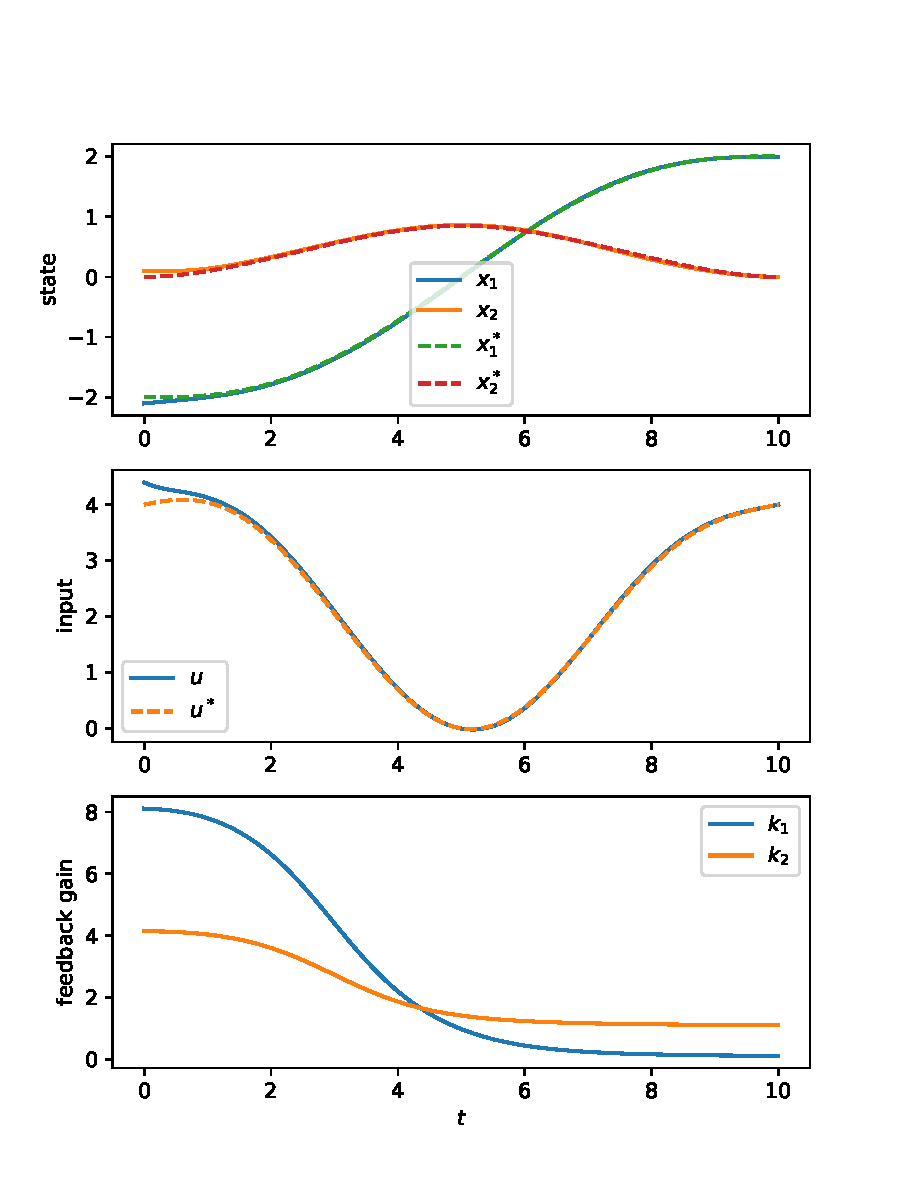
\includegraphics[scale=1]{img/ludyk_ltv.pdf}
    \caption{Closed loop simulation of trajectory tracking, controller designed for linear time-variant system obtained from linearizing along reference trajectory}
    \label{fig:ludyk_ltv}
\end{figure}

Unfortunately the final state trajectory is visually indistinguishable from the previous result.
Still, for less benevolent systems than this academic example this method is the safer option, as it is applicable whenever the feedforward control is good enough to not deviate from the reference too far.

\FloatBarrier
\section{Cart-Pole System}

To demonstrate the broader applicability of this controller design, it will now be implemented for a second example.
The chosen system is the cart-pole inverse pendulum seen in Figure~\ref{fig:pendulum_sketch}.

\begin{figure}[ht]
    \centering
    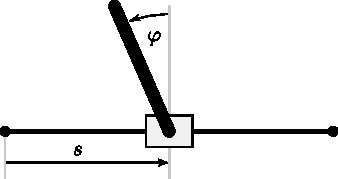
\includegraphics[scale=1]{img/pendulum.pdf}
    \caption{Cart-pole inverse pendulum}
    \label{fig:pendulum_sketch}
\end{figure}

The state vector~$x$ consists of the cart position~$s$ and the angle~$\varphi$ as well as their first time derivatives, so
$$
x = \begin{pmatrix}x_1\\x_2\\x_3\\x_4\end{pmatrix} := \begin{pmatrix}s\\\dot s\\\varphi\\\dot\varphi\end{pmatrix}\, ,
$$
while the input is the cart acceleration~$u = a$.
The system equation already in state-space form then is:
$$
\dot x = F(x, u) = \begin{pmatrix}x_2\\u\\x_4\\\frac{1}{l}(g \sin x_3+u\cos x_3)\end{pmatrix}\, .
$$
From differentiation follows for the linearized system matrices
$$
A(x^*, u^*) := \left.\frac{\partial F}{\partial x}\right\vert_{(x^*, u^*)}= \begin{pmatrix}0 & 1 & 0 & 0\\0 & 0 & 0 & 0\\0 & 0 & 0 & 1\\0 & 0 & \frac{1}{l}(g \cos x_3 - u \sin x_3) & 0\end{pmatrix}
$$
and
$$
B(x^*, u^*) := \left.\frac{\partial F}{\partial u}\right\vert_{(x^*, u^*)}= \begin{pmatrix}0\\1\\0\\\frac{\cos x_3}{l}\end{pmatrix}\, .
$$
Converted to \py this system description becomes:
\luainputlisting{../sim/01_lqr_pendulum.py}{defsystem}

The task will be a swingup of the  pendulum, meaning that it should move from the lower equilibrium~$x(0)=(0, 0, \pi, 0)$ to the upper equilibrium~$x(t_f) = (0, 0, 0, 0)$.
How to plan trajectories like this is a separate topic that will not be discussed here.
For now, assume that the necessary trajectory data is somehow known.

The code trajectory contains a file \texttt{pendulum.csv} with this trajectory.
The first column is a time vector with fixed step width of 10\,ms, the following four columns describe the state at each time step and the last column is the input signal.
In \py this data can be loaded like this:
\luainputlisting{../sim/01_lqr_pendulum.py}{loadcsv}
All the other code doing the controller design and the simulation can be reused.

Because the dynamics at the upper and lower position are obviously very different, it is to be expected that an LQR designed for time-invariant system approximation will struggle.
If it assumes the system to be at the lower position it will not be able to stabilize it when it's actually at the upper one.
Reversely, designing it for the upper position makes tracking during the swingup difficult.
This last case was simulated in Figure~\ref{fig:pendulum_lti}.
Even though the feedforward control was very precise, tracking does not work at all.

\begin{figure}[ht]
    \centering
    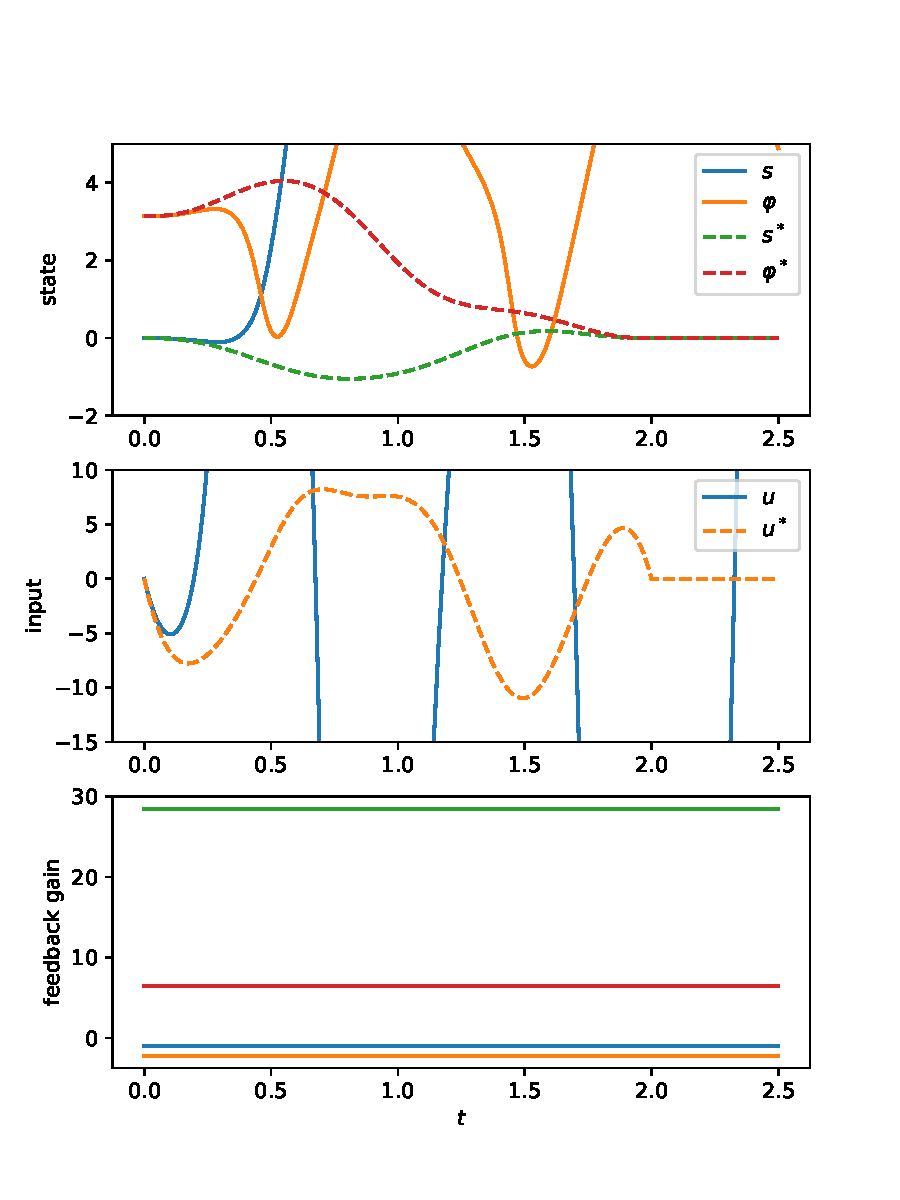
\includegraphics[scale=1]{img/pendulum_lti.pdf}
    \caption{Pendulum swingup, LQR designed for linear time-invariant system at the upper equilibrium}
    \label{fig:pendulum_lti}
\end{figure}

In the previous example, this issues could be alleviated with the workaround of retuning the controller at every time step.
Figure~\ref{fig:pendulum_pseudoltv} shows how this can also fail when the system is slightly more involved.
Even though the pendulum arm reaches the upper position and stays there, the cart position starts drifting off halfway through the trajectory.

\begin{figure}[ht]
    \centering
    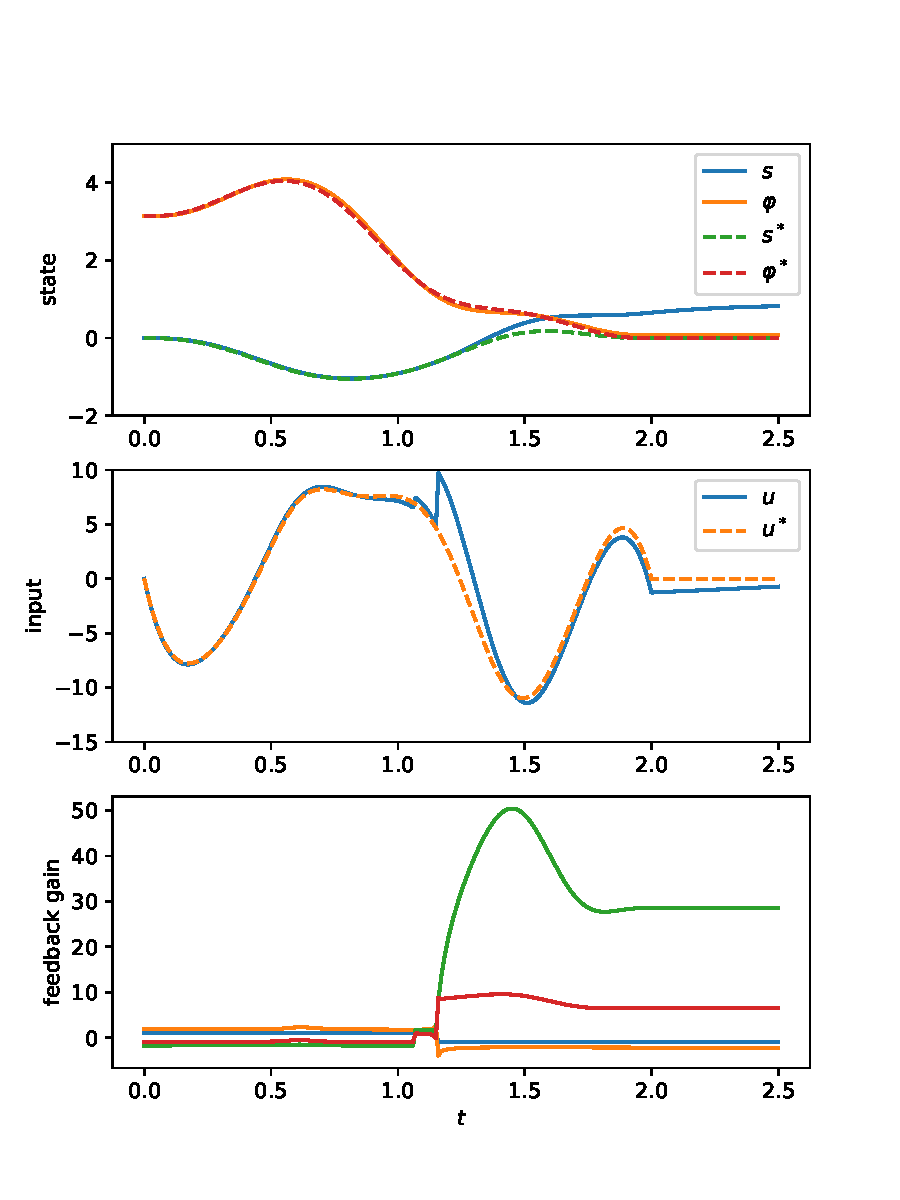
\includegraphics[scale=1]{img/pendulum_pseudoltv.pdf}
    \caption{Pendulum swingup, LQR is retuned at every time step for the current desired state}
    \label{fig:pendulum_pseudoltv}
\end{figure}

Finally, an LQR properly designed for a linear time-variant system approximation was used in Figure~\ref{fig:pendulum_ltv}.
At least in simulation tracking works with issues.
Both during swingup and while remaining at the upper equilibrium the state follows the reference well.
Furthermore the difference of the feedback matrix~$K(t)$ between this version and the previous ad-hoc solution now becomes obvious.

\begin{figure}[ht]
    \centering
    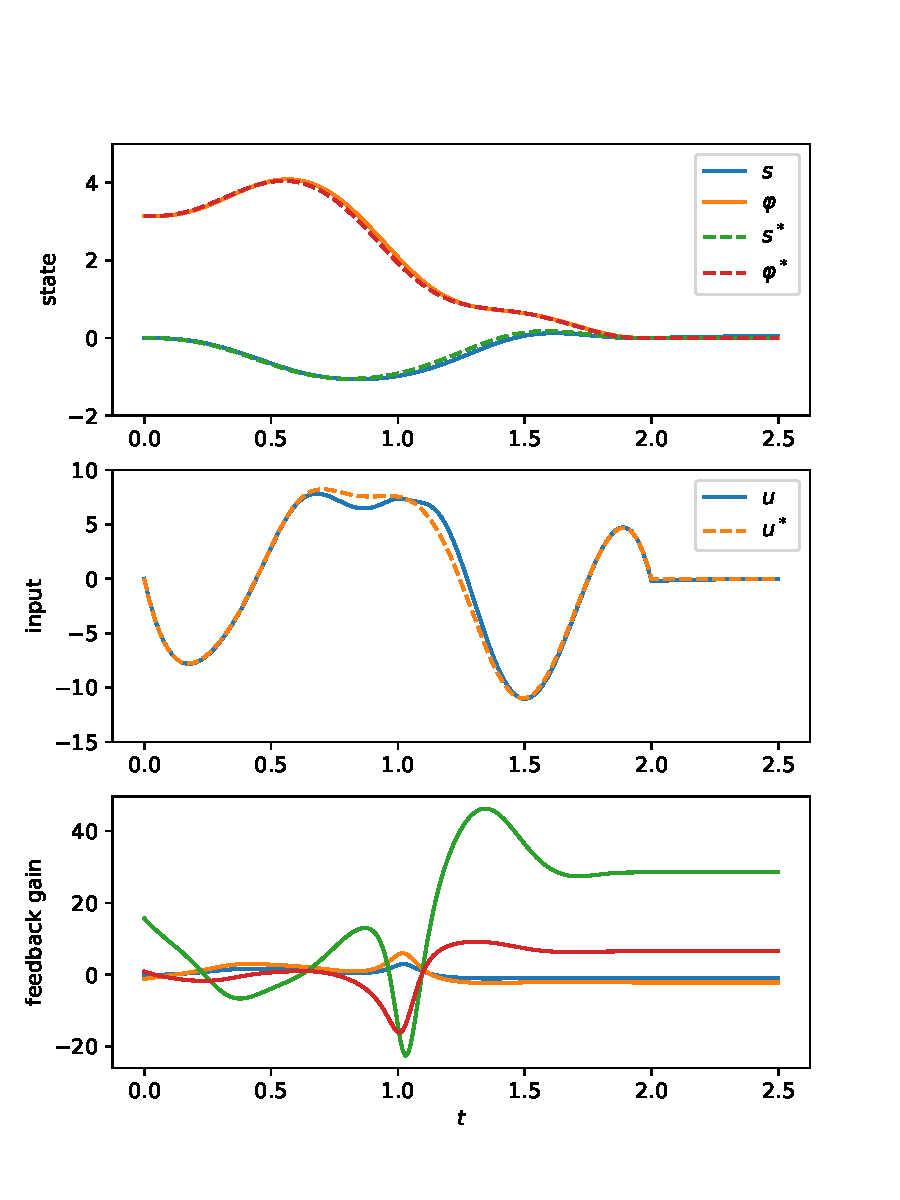
\includegraphics[scale=1]{img/pendulum_ltv.pdf}
    \caption{Pendulum swingup, LQR designed for linear time-variant system approximation}
    \label{fig:pendulum_ltv}
\end{figure}

\printglossaries
%\printbibliography

\end{document}

%%% Local Variables:
%%% mode: latex
%%% TeX-master: t
%%% End: